\documentclass[10pt]{beamer}
\usetheme{Madrid}
\usecolortheme{default}
\usepackage{graphicx}
\usepackage{amsmath,amssymb}
\usepackage{bm}
\usepackage{tikz}

\usetikzlibrary{shapes,arrows,positioning,calc}
\tikzset{
	block/.style = {draw, rectangle, minimum height=1.2cm, minimum width=2cm, align=center},
	sum/.style = {draw, circle, node distance=1cm},
	input/.style = {coordinate},
	output/.style = {coordinate},
	spring/.style = {decorate, decoration={coil, amplitude=3pt, segment length=3pt}},
}
\usepackage{booktabs}

% Title page info
\title{Robot Motion and Force Control}
\subtitle{From Independent Joints to Operational Space and Interaction Control}
\author{Your Name}
\institute{Your Institution}
\date{\today}

% Define commands for robot dynamics
\newcommand{\vect}[1]{\boldsymbol{#1}}
\newcommand{\M}{\vect{M}}
\newcommand{\C}{\vect{C}}
\newcommand{\g}{\vect{g}}
\newcommand{\q}{\vect{q}}
\newcommand{\qd}{\vect{q}_d}
\newcommand{\qdot}{\dot{\vect{q}}}
\newcommand{\qddot}{\ddot{\vect{q}}}
\newcommand{\tauvec}{\vect{\tau}}
\newcommand{\x}{\vect{x}}
\newcommand{\xd}{\vect{x}_d}
\newcommand{\J}{\vect{J}}
\newcommand{\F}{\vect{F}}
\newcommand{\Kp}{\vect{K}_p}
\newcommand{\Kd}{\vect{K}_d}
\newcommand{\Ki}{\vect{K}_i}

\begin{document}


\section{Actuators in Robotics}
\begin{frame}{Actuators: The "Muscles" of Robots}
	\begin{block}{Definition}
		Actuators convert energy into mechanical motion. They provide the \textbf{force/torque} to move robot joints.
	\end{block}
	
	\begin{columns}
		\begin{column}{0.5\textwidth}
			\begin{exampleblock}{Main Types}
				\begin{enumerate}
					\item \textbf{Electric Motors}
					\begin{itemize}
						\footnotesize
						\item DC Motors (Brushed/Brushless)
						\item Stepper Motors
						\item Servo Motors
					\end{itemize}
					\item \textbf{Hydraulic Actuators}
					\item \textbf{Pneumatic Actuators}
					\item \textbf{Smart Material Actuators}
					\begin{itemize}
						\footnotesize
						\item Piezoelectric
						\item Shape Memory Alloys
					\end{itemize}
				\end{enumerate}
			\end{exampleblock}
		\end{column}
		
		\begin{column}{0.5\textwidth}
			\begin{center}
				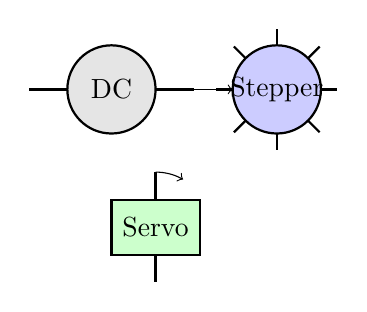
\begin{tikzpicture}[scale=0.7]
					% DC Motor
					\draw[thick, fill=gray!20] (0,0) circle (0.8);
					\draw[thick] (-0.8,0) -- (-1.5,0);
					\draw[thick] (0.8,0) -- (1.5,0);
					\draw[->] (1.5,0) -- (2.2,0);
					\node at (0,0) {DC};
					
					% Stepper
					\draw[thick, fill=blue!20] (3,0) circle (0.8);
					\foreach \i in {0,45,90,135,180,225,270,315}
					\draw[thick] (3,0) ++(\i:0.8) -- ++(\i:0.3);
					\node at (3,0) {Stepper};
					
					% Servo
					\draw[thick, fill=green!20] (0,-2) rectangle (1.6,-3);
					\draw[thick] (0.8,-2) -- (0.8,-1.5);
					\draw[thick] (0.8,-3) -- (0.8,-3.5);
					\draw[->] (0.8,-1.5) arc (90:60:1);
					\node at (0.8,-2.5) {Servo};
				\end{tikzpicture}
			\end{center}
		\end{column}
	\end{columns}
\end{frame}

\begin{frame}{Electric Motors: The Most Common Choice}
	\begin{table}[h]
		\centering
		\begin{tabular}{p{0.3\textwidth} p{0.3\textwidth} p{0.3\textwidth}}
			\toprule
			\textbf{Type} & \textbf{Advantages} & \textbf{Disadvantages} \\
			\midrule
			\textbf{DC Brushed} & 
			\begin{itemize}
				\footnotesize
				\item Simple control
				\item Low cost
				\item High torque at low speed
			\end{itemize} &
			\begin{itemize}
				\footnotesize
				\item Brush wear
				\item EMI
				\item Maintenance
			\end{itemize} \\
			
			\textbf{DC Brushless} &
			\begin{itemize}
				\footnotesize
				\item High efficiency
				\item Long life
				\item High power density
			\end{itemize} &
			\begin{itemize}
				\footnotesize
				\item Complex control
				\item Higher cost
				\item Needs encoder
			\end{itemize} \\
			
			\textbf{Stepper} &
			\begin{itemize}
				\footnotesize
				\item Open-loop control
				\item Good position accuracy
				\item High holding torque
			\end{itemize} &
			\begin{itemize}
				\footnotesize
				\item Resonance issues
				\item Low efficiency
				\item Can lose steps
			\end{itemize} \\
			\bottomrule
		\end{tabular}
	\end{table}
	
	\begin{block}{Key Parameters}
		\begin{itemize}
			\item \textbf{Torque Constant} ($K_t$): Nm/A
			\item \textbf{Back-EMF Constant} ($K_e$): V/(rad/s)
			\item \textbf{Rated Torque/Speed}
			\item \textbf{Power Density}: W/kg
		\end{itemize}
	\end{block}
\end{frame}

\begin{frame}{Hydraulic vs. Pneumatic Actuators}
	\begin{columns}
		\begin{column}{0.48\textwidth}
			\begin{block}{Hydraulic Actuators}
				\begin{center}
					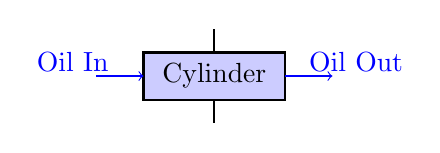
\begin{tikzpicture}[scale=0.6]
						\draw[thick, fill=blue!20] (0,0) rectangle (3,1);
						\draw[thick] (1.5,1) -- (1.5,1.5);
						\draw[thick] (1.5,0) -- (1.5,-0.5);
						\draw[->, blue] (-1,0.5) -- (0,0.5);
						\draw[->, blue] (3,0.5) -- (4,0.5);
						\node at (1.5,0.5) {Cylinder};
						\node[blue] at (-1.5,0.8) {Oil In};
						\node[blue] at (4.5,0.8) {Oil Out};
					\end{tikzpicture}
				\end{center}
				\begin{itemize}
					\item \textbf{Very high force/torque}
					\item Good stiffness
					\item Can be leaky, messy
					\item Needs pump, reservoir
					\item \textbf{Applications:} Excavators, heavy lifting
				\end{itemize}
			\end{block}
		\end{column}
		
		\begin{column}{0.48\textwidth}
			\begin{block}{Pneumatic Actuators}
				\begin{center}
					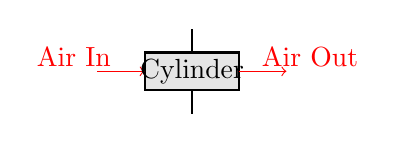
\begin{tikzpicture}[scale=0.6]
						\draw[thick, fill=gray!20] (0,0) rectangle (2,0.8);
						\draw[thick] (1,0.8) -- (1,1.3);
						\draw[thick] (1,0) -- (1,-0.5);
						\draw[->, red] (-1,0.4) -- (0,0.4);
						\draw[->, red] (2,0.4) -- (3,0.4);
						\node at (1,0.4) {Cylinder};
						\node[red] at (-1.5,0.7) {Air In};
						\node[red] at (3.5,0.7) {Air Out};
					\end{tikzpicture}
				\end{center}
				\begin{itemize}
					\item \textbf{Fast, clean}
					\item Lower force than hydraulic
					\item Compressible $\Rightarrow$ less stiff
					\item Needs compressor, dryer
					\item \textbf{Applications:} Pick-and-place, assembly
				\end{itemize}
			\end{block}
		\end{column}
	\end{columns}
	
	\vspace{5mm}
	\begin{alertblock}{Modern Trend: Electro-Hydrostatic Actuators (EHA)}
		Electric motor + pump + cylinder in one package. Best of both worlds!
	\end{alertblock}
\end{frame}

\section{Sensors for Motion Sensing}
\begin{frame}{Sensors: The "Senses" of Robots}
	\begin{block}{Motion Sensing Hierarchy}
		\begin{itemize}
			\item \textbf{Joint-level sensing:} Where is each joint?
			\item \textbf{End-effector sensing:} Where is the tool?
			\item \textbf{Environment sensing:} What's around the robot?
		\end{itemize}
	\end{block}
	
	\begin{columns}
		\begin{column}{0.5\textwidth}
			\begin{exampleblock}{Position/Velocity Sensors}
				\begin{itemize}
					\item \textbf{Encoders}
					\begin{itemize}
						\footnotesize
						\item Incremental
						\item Absolute
					\end{itemize}
					\item \textbf{Potentiometers}
					\item \textbf{Resolvers}
					\item \textbf{LVDT/RVDT}
					\item \textbf{Hall Effect Sensors}
				\end{itemize}
			\end{exampleblock}
		\end{column}
		
		\begin{column}{0.5\textwidth}
			\begin{exampleblock}{Force/Torque Sensors}
				\begin{itemize}
					\item \textbf{Strain Gauges}
					\item \textbf{Load Cells}
					\item \textbf{Force-Torque Sensors}
					\item \textbf{Tactile Sensors}
					\item \textbf{Pressure Sensors}
				\end{itemize}
			\end{exampleblock}
		\end{column}
	\end{columns}
\end{frame}

\begin{frame}{Encoders: The Workhorse of Robot Sensing}
	\begin{columns}
		\begin{column}{0.5\textwidth}
			\begin{block}{Incremental Encoders}
				\begin{center}
					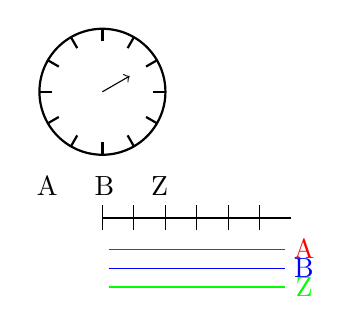
\begin{tikzpicture}[scale=0.8]
						\draw[thick] (0,0) circle (1);
						\foreach \i in {0,30,...,330} {
							\draw[thick] (\i:0.8) -- (\i:1);
						}
						\draw[->] (0,0) -- (30:0.5);
						\node at (0,-1.5) {A \quad B \quad Z};
						\draw[thick] (0,-2) -- (3,-2);
						\foreach \i in {0,0.5,1,1.5,2,2.5} {
							\draw (\i,-1.8) -- (\i,-2.2);
						}
						\draw[red] (0.1,-2.5) -- (2.9,-2.5);
						\draw[blue] (0.1,-2.8) -- (2.9,-2.8);
						\draw[green] (0.1,-3.1) -- (2.9,-3.1);
						\node[red] at (3.2,-2.5) {A};
						\node[blue] at (3.2,-2.8) {B};
						\node[green] at (3.2,-3.1) {Z};
					\end{tikzpicture}
				\end{center}
				\begin{itemize}
					\footnotesize
					\item Pulses per revolution (PPR)
					\item Channels A, B (quadrature)
					\item Index channel Z
					\item Need homing
				\end{itemize}
			\end{block}
		\end{column}
		
		\begin{column}{0.5\textwidth}
			\begin{block}{Absolute Encoders}
				\begin{center}
					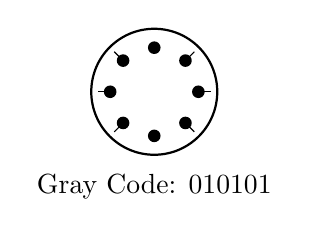
\begin{tikzpicture}[scale=0.8]
						\draw[thick] (0,0) circle (1);
						\foreach \i in {0,45,...,315} {
							\fill (\i:0.7) circle (0.1);
						}
						\draw (0:0.7) -- (0:0.9);
						\draw (45:0.7) -- (45:0.9);
						\draw (135:0.7) -- (135:0.9);
						\draw (180:0.7) -- (180:0.9);
						\draw (225:0.7) -- (225:0.9);
						\draw (315:0.7) -- (315:0.9);
						\node at (0,-1.5) {Gray Code: 010101};
					\end{tikzpicture}
				\end{center}
				\begin{itemize}
					\footnotesize
					\item Unique code per position
					\item No homing needed
					\item Single-turn vs multi-turn
					\item More expensive
				\end{itemize}
			\end{block}
		\end{column}
	\end{columns}
	
	\begin{alertblock}{Encoder Resolution}
		$\Delta\theta = \frac{360^\circ}{\text{PPR} \times 4}$ (with quadrature decoding)
	\end{alertblock}
\end{frame}

\begin{frame}{Force/Torque and Vision Sensors}
	\begin{columns}
		\begin{column}{0.48\textwidth}
			\begin{block}{Force-Torque Sensors}
				\begin{center}
					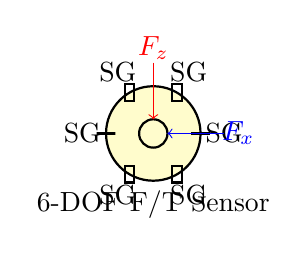
\begin{tikzpicture}[scale=0.6]
						\draw[thick, fill=yellow!20] (0,0) circle (1);
						\foreach \i in {0,60,...,300} {
							\draw[thick] (\i:0.8) rectangle (\i:1.2);
							\node at (\i:1.5) {SG};
						}
						\draw[thick] (0,0) circle (0.3);
						\draw[->, red] (0,1.5) -- (0,0.3);
						\draw[->, blue] (1.5,0) -- (0.3,0);
						\node[red] at (0,1.8) {$F_z$};
						\node[blue] at (1.8,0) {$F_x$};
						\node at (0,-1.5) {6-DOF F/T Sensor};
					\end{tikzpicture}
				\end{center}
				\begin{itemize}
					\footnotesize
					\item Measures $F_x, F_y, F_z, M_x, M_y, M_z$
					\item Strain gauge based
					\item Mounted at wrist
					\item Critical for force control
				\end{itemize}
			\end{block}
		\end{column}
		
		\begin{column}{0.48\textwidth}
			\begin{block}{Vision Systems}
				\begin{center}
					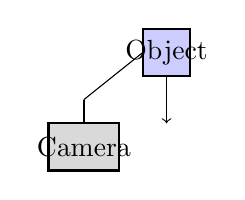
\begin{tikzpicture}[scale=0.6]
						\draw[thick, fill=gray!30] (0,0) rectangle (1.5,1);
						\draw[thick] (0.75,1) -- (0.75,1.5);
						\node at (0.75,0.5) {Camera};
						\draw (0.75,1.5) -- (2,2.5);
						\draw[thick, fill=blue!20] (2,2) rectangle (3,3);
						\node at (2.5,2.5) {Object};
						\draw[->] (2.5,2) -- (2.5,1);
					\end{tikzpicture}
				\end{center}
				\begin{itemize}
					\footnotesize
					\item 2D/3D vision
					\item Eye-in-hand vs fixed
					\item For guidance, inspection
					\item Often with LED lighting
				\end{itemize}
			\end{block}
			
			\begin{block}{Other Sensors}
				\begin{itemize}
					\footnotesize
					\item \textbf{Proximity:} Inductive, capacitive
					\item \textbf{LIDAR:} For mapping, navigation
					\item \textbf{IMU:} Accelerometer, gyro
					\item \textbf{Torque Sensors:} In joint
				\end{itemize}
			\end{block}
		\end{column}
	\end{columns}
\end{frame}

\section{Motion Transmission Mechanisms}
\begin{frame}{Why Transmission Mechanisms?}
	\begin{block}{The Motor-Robot Interface Problem}
		\begin{itemize}
			\item Motors have \textbf{high speed, low torque}
			\item Robots need \textbf{low speed, high torque}
			\item Need \textbf{gear reduction} (typically 50:1 to 200:1)
			\item Also need to \textbf{transmit motion} to different locations
		\end{itemize}
	\end{block}
	
	\begin{columns}
		\begin{column}{0.5\textwidth}
			\begin{exampleblock}{Common Mechanisms}
				\begin{enumerate}
					\item Gears (Spur, Planetary, Harmonic)
					\item Belts and Pulleys
					\item Chains and Sprockets
					\item Lead/Ball Screws
					\item Cable Drives
					\item Linkages
				\end{enumerate}
			\end{exampleblock}
		\end{column}
		
		\begin{column}{0.5\textwidth}
			\begin{center}
				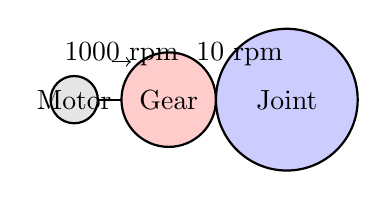
\begin{tikzpicture}[scale=0.6]
					% Motor to gear reduction
					\draw[thick, fill=gray!20] (0,0) circle (0.5);
					\node at (0,0) {Motor};
					\draw[thick] (0.5,0) -- (1.5,0);
					\draw[thick, fill=red!20] (2,0) circle (1);
					\node at (2,0) {Gear};
					\draw[thick] (3,0) -- (4,0);
					\draw[thick, fill=blue!20] (4.5,0) circle (1.5);
					\node at (4.5,0) {Joint};
					\node[above] at (1,0.5) {$1000$ rpm};
					\node[above] at (3.5,0.5) {$10$ rpm};
					\draw[->] (0.8,0.8) -- (1.2,0.8);
				\end{tikzpicture}
			\end{center}
			\begin{alertblock}{Key Metrics}
				\begin{itemize}
					\footnotesize
					\item \textbf{Gear Ratio} ($N$)
					\item \textbf{Efficiency} ($\eta$)
					\item \textbf{Backlash}
					\item \textbf{Stiffness}
					\item \textbf{Mass/Inertia}
				\end{itemize}
			\end{alertblock}
		\end{column}
	\end{columns}
\end{frame}

\begin{frame}{Gear Mechanisms}
	\begin{columns}
		\begin{column}{0.33\textwidth}
			\begin{block}{Spur Gears}
				\begin{center}
					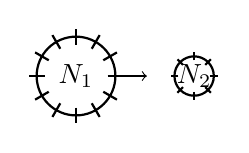
\begin{tikzpicture}[scale=0.5]
						\draw[thick] (0,0) circle (1);
						\foreach \i in {0,30,...,330} {
							\draw[thick] (\i:0.8) -- (\i:1.2);
						}
						\draw[thick] (3,0) circle (0.5);
						\foreach \i in {0,45,...,315} {
							\draw[thick] (3,0) ++(\i:0.4) -- ++(\i:0.2);
						}
						\draw[->] (1.2,0) -- (1.8,0);
						\node at (0,0) {$N_1$};
						\node at (3,0) {$N_2$};
					\end{tikzpicture}
				\end{center}
				\begin{itemize}
					\footnotesize
					\item Parallel shafts
					\item $N = N_2/N_1$
					\item Simple, efficient
					\item Can have backlash
				\end{itemize}
			\end{block}
		\end{column}
		
		\begin{column}{0.33\textwidth}
			\begin{block}{Planetary Gears}
				\begin{center}
					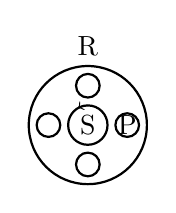
\begin{tikzpicture}[scale=0.5]
						\draw[thick] (0,0) circle (1.5); % Ring
						\draw[thick] (0,0) circle (0.5); % Sun
						\draw[thick] (1,0) circle (0.3); % Planet
						\draw[thick] (-1,0) circle (0.3);
						\draw[thick] (0,1) circle (0.3);
						\draw[thick] (0,-1) circle (0.3);
						\node at (0,0) {S};
						\node at (1,0) {P};
						\node at (0,2) {R};
						\draw[->] (0,0.5) arc (90:120:0.5);
					\end{tikzpicture}
				\end{center}
				\begin{itemize}
					\footnotesize
					\item High reduction in small package
					\item Multiple power paths
					\item High torque density
					\item Complex, expensive
				\end{itemize}
			\end{block}
		\end{column}
		
		\begin{column}{0.33\textwidth}
			\begin{block}{Harmonic Drive}
				\begin{center}
					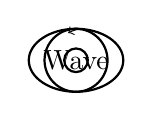
\begin{tikzpicture}[scale=0.5]
						\draw[thick, ellipse] (0,0) circle (1.2 and 0.8);
						\draw[thick] (0,0) circle (0.8);
						\draw[thick] (0,0) circle (0.3);
						\node at (0,0) {Wave};
						\draw[->] (0.2,0.8) arc (90:120:0.8);
					\end{tikzpicture}
				\end{center}
				\begin{itemize}
					\footnotesize
					\item \textbf{Zero backlash}
					\item Very high ratios (50:1 to 320:1)
					\item High precision
					\item Limited torque, expensive
					\item Used in robot wrist joints
				\end{itemize}
			\end{block}
		\end{column}
	\end{columns}
	
	\vspace{3mm}
	\begin{alertblock}{Gear Ratio Effects}
		\begin{itemize}
			\item \textbf{Torque:} $\tau_{out} = N \eta \tau_{in}$
			\item \textbf{Speed:} $\omega_{out} = \omega_{in}/N$
			\item \textbf{Reflected Inertia:} $J_{reflected} = J_{motor} \times N^2$
		\end{itemize}
	\end{alertblock}
\end{frame}

\begin{frame}{Belts, Pulleys, and Other Transmissions}
	\begin{columns}
		\begin{column}{0.48\textwidth}
			\begin{block}{Timing Belts \& Pulleys}
				\begin{center}
					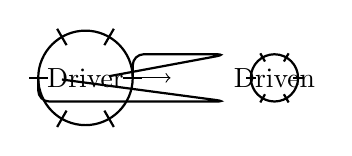
\begin{tikzpicture}[scale=0.6]
						\draw[thick] (0,0) circle (1);
						\foreach \i in {0,60,...,300} {
							\draw[thick] (\i:0.8) -- (\i:1.2);
						}
						\draw[thick] (4,0) circle (0.5);
						\foreach \i in {0,60,...,300} {
							\draw[thick] (4,0) ++(\i:0.4) -- ++(\i:0.2);
						}
						\draw[thick, rounded corners] (0:1) -- (1,0.5) -- (3,0.5) -- (4:0.5);
						\draw[thick, rounded corners] (180:1) -- (-1,-0.5) -- (3,-0.5) -- (184:0.5);
						\node at (0,0) {Driver};
						\node at (4,0) {Driven};
						\draw[->] (1.2,0) -- (1.8,0);
					\end{tikzpicture}
				\end{center}
				\begin{itemize}
					\footnotesize
					\item \textbf{Synchronous} (no slip)
					\item Good for long distances
					\item Low backlash
					\item Needs tensioning
				\end{itemize}
			\end{block}
			
			\begin{block}{Ball Screws}
				\begin{center}
					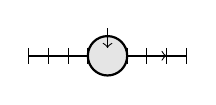
\begin{tikzpicture}[scale=0.5]
						\draw[thick] (0,0) -- (4,0);
						\foreach \x in {0,0.5,...,4} {
							\draw (\x,0.2) -- (\x,-0.2);
						}
						\draw[thick, fill=gray!20] (2,0) circle (0.5);
						\draw[->] (2,0.7) -- (2,0.2);
						\draw[->] (2.5,0) -- (3.5,0);
					\end{tikzpicture}
				\end{center}
				\begin{itemize}
					\footnotesize
					\item Converts rotation to translation
					\item High efficiency (90\%+)
					\item Zero backlash possible
					\item Used in linear axes
				\end{itemize}
			\end{block}
		\end{column}
		
		\begin{column}{0.48\textwidth}
			\begin{block}{Cable Drives}
				\begin{center}
					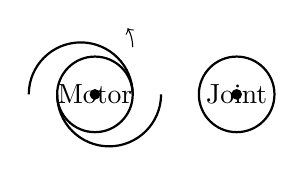
\begin{tikzpicture}[scale=0.6]
						\draw[thick] (0,0) circle (0.8);
						\draw[thick] (3,0) circle (0.8);
						\draw[thick] (0.8,0) arc (0:180:1.1);
						\draw[thick] (-0.8,0) arc (180:360:1.1);
						\draw[fill=black] (0,0) circle (0.1);
						\draw[fill=black] (3,0) circle (0.1);
						\node at (0,0) {Motor};
						\node at (3,0) {Joint};
						\draw[->] (0.8,1) arc (0:30:0.8);
					\end{tikzpicture}
				\end{center}
				\begin{itemize}
					\footnotesize
					\item \textbf{Remote actuation}
					\item Low inertia at moving part
					\item Used in surgical robots
					\item Needs tensioning, can stretch
				\end{itemize}
			\end{block}
			
			\begin{block}{Direct Drive}
				\begin{center}
					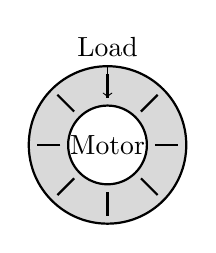
\begin{tikzpicture}[scale=0.5]
						\draw[thick, fill=gray!30] (0,0) circle (2);
						\draw[thick, fill=white] (0,0) circle (1);
						\foreach \i in {0,45,...,315} {
							\draw[thick] (\i:1.2) -- (\i:1.8);
						}
						\node at (0,0) {Motor};
						\node at (0,2.5) {Load};
						\draw[->] (0,2) -- (0,1.2);
					\end{tikzpicture}
				\end{center}
				\begin{itemize}
					\footnotesize
					\item \textbf{No gears} - motor directly connected
					\item Zero backlash, high stiffness
					\item Needs high-torque motor
					\item Used in precision applications
				\end{itemize}
			\end{block}
		\end{column}
	\end{columns}
\end{frame}

\section{End Effectors for Industrial Robots}
\begin{frame}{End Effectors: The "Hands" of Robots}
	\begin{block}{Definition}
		End effectors are devices mounted at the robot wrist that \textbf{interact with the environment} to perform tasks.
	\end{block}
	
	\begin{columns}
		\begin{column}{0.5\textwidth}
			\begin{exampleblock}{Two Main Categories}
				\begin{enumerate}
					\item \textbf{Grippers}
					\begin{itemize}
						\footnotesize
						\item Mechanical
						\item Vacuum
						\item Magnetic
						\item Adhesive
					\end{itemize}
					\item \textbf{Tools}
					\begin{itemize}
						\footnotesize
						\item Welding
						\item Painting
						\item Drilling
						\item Dispensing
					\end{itemize}
				\end{enumerate}
			\end{exampleblock}
			\end{column>
				
				\begin{column}{0.5\textwidth}
					\begin{center}
						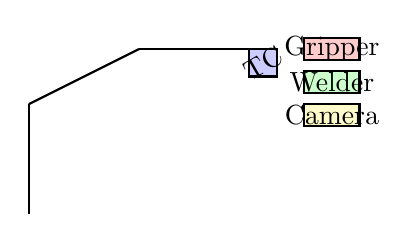
\begin{tikzpicture}[scale=0.7]
							% Robot arm
							\draw[thick] (0,0) -- (0,2);
							\draw[thick] (0,2) -- (2,3);
							\draw[thick] (2,3) -- (4,3);
							
							% Tool changer
							\draw[thick, fill=blue!20] (4,3) rectangle (4.5,2.5);
							\node[rotate=30] at (4.25,2.75) {TC};
							
							% Different end effectors
							\draw[thick, fill=red!20] (5,3.2) rectangle (6,2.8);
							\node at (5.5,3) {Gripper};
							
							\draw[thick, fill=green!20] (5,2.6) rectangle (6,2.2);
							\node at (5.5,2.4) {Welder};
							
							\draw[thick, fill=yellow!20] (5,2.0) rectangle (6,1.6);
							\node at (5.5,1.8) {Camera};
						\end{tikzpicture}
					\end{center}
				\end{column}
			\end{columns}
			
			\begin{alertblock}{Tool Changers}
				Allow one robot to use multiple end effectors automatically. Critical for flexible automation.
			\end{alertblock}
		\end{frame}
		
		\begin{frame}{Mechanical Grippers: The Most Common Type}
			\begin{columns}
				\begin{column}{0.48\textwidth}
					\begin{block}{Two-Finger Grippers}
						\begin{center}
							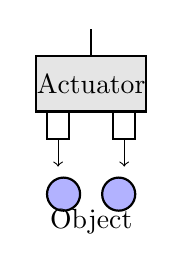
\begin{tikzpicture}[scale=0.7]
								\draw[thick, fill=gray!20] (0,0) rectangle (2,1);
								\draw[thick] (1,1) -- (1,1.5);
								\draw[thick] (0.2,0) rectangle (0.6,-0.5);
								\draw[thick] (1.4,0) rectangle (1.8,-0.5);
								\draw[->] (0.4,-0.5) -- (0.4,-1);
								\draw[->] (1.6,-0.5) -- (1.6,-1);
								\node at (1,0.5) {Actuator};
								\draw[thick, fill=blue!30] (0.5,-1.5) circle (0.3);
								\draw[thick, fill=blue!30] (1.5,-1.5) circle (0.3);
								\node at (1,-2) {Object};
							\end{tikzpicture}
						\end{center}
						\begin{itemize}
							\footnotesize
							\item Parallel jaw
							\item Angular jaw
							\item Self-centering
							\item Actuation: Pneumatic, electric, hydraulic
						\end{itemize}
					\end{block}
					\end{column>
						
						\begin{column}{0.48\textwidth}
							\begin{block}{Three-Finger Grippers}
								\begin{center>
									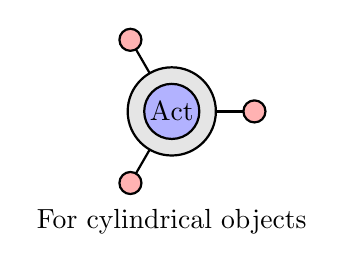
\begin{tikzpicture}[scale=0.7]
										\draw[thick, fill=gray!20] (0,0) circle (0.8);
										\foreach \i in {0,120,240} {
											\draw[thick] (\i:0.8) -- (\i:1.5);
											\draw[thick, fill=red!30] (\i:1.5) circle (0.2);
										}
										\draw[thick, fill=blue!30] (0,0) circle (0.5);
										\node at (0,0) {Act};
										\node at (0,-2) {For cylindrical objects};
									\end{tikzpicture}
									\end{center>
										\begin{itemize}
											\footnotesize
											\item Better centering
											\item More contact points
											\item Can grip irregular shapes
											\item More complex mechanism
										\end{itemize}
										\end{block>
										\end{column}
										\end{columns>
											
											\vspace{3mm}
											\begin{block}{Gripper Specifications}
												\begin{itemize}
													\item \textbf{Force:} 10N to 1000N+
													\item \textbf{Stroke:} Opening width
													\item \textbf{Repeatability:} Typically ±0.02mm
													\item \textbf{Weight:} Affects robot payload
													\item \textbf{Fingers:} Customizable for parts
												\end{itemize}
											\end{block}
										\end{frame}
										
										\begin{frame}{Vacuum and Specialized Grippers}
											\begin{columns}
												\begin{column}{0.48\textwidth}
													\begin{block}{Vacuum Grippers (Suction Cups)}
														\begin{center>
															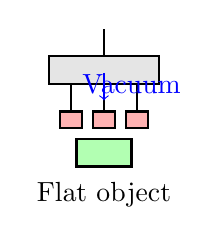
\begin{tikzpicture}[scale=0.7]
																\draw[thick, fill=gray!20] (0,0) rectangle (2,0.5);
																\draw[thick] (1,0.5) -- (1,1);
																\foreach \x in {0.4,1,1.6} {
																	\draw[thick] (\x,0) -- (\x,-0.5);
																	\draw[thick, fill=red!30] (\x-0.2,-0.5) rectangle (\x+0.2,-0.8);
																}
																\draw[->, blue] (1,0.2) -- (1,-0.3);
																\node[blue] at (1.5,0) {Vacuum};
																\draw[thick, fill=green!30] (0.5,-1.5) rectangle (1.5,-1);
																\node at (1,-2) {Flat object};
															\end{tikzpicture}
															\end{center>
																\begin{itemize}
																	\footnotesize
																	\item For \textbf{flat, smooth} surfaces
																	\item Multiple cups for large objects
																	\item \textbf{Venturi} or vacuum pump
																	\item Fast pick-and-place
																	\item Limited to non-porous materials
																\end{itemize}
																\end{block>
																	\end{column>
																		
																		\begin{column}{0.48\textwidth}
																			\begin{block}{Magnetic Grippers}
																				\begin{center>
																					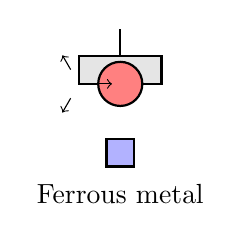
\begin{tikzpicture}[scale=0.7]
																						\draw[thick, fill=gray!20] (0,0) rectangle (1.5,0.5);
																						\draw[thick] (0.75,0.5) -- (0.75,1);
																						\draw[thick, fill=red!50] (0.75,0) circle (0.4);
																						\foreach \i in {0,120,240} {
																							\draw[->] (\i:0.3) -- (\i:0.6);
																						}
																						\draw[thick, fill=blue!30] (0.5,-1) rectangle (1,-1.5);
																						\node at (0.75,-2) {Ferrous metal};
																					\end{tikzpicture}
																					\end{center>
																						\begin{itemize}
																							\footnotesize
																							\item For \textbf{ferrous metals}
																							\item Permanent or electromagnetic
																							\item No power needed for holding (permanent)
																							\item Can pick through paint/coating
																						\end{itemize}
																						\end{block>
																							
																							\begin{block}{Specialized Grippers}
																								\begin{itemize}
																									\footnotesize
																									\item \textbf{Needle grippers:} For textiles
																									\item \textbf{Inflatable grippers:} For fragile items
																									\item \textbf{Electrostatic:} For wafers, glass
																									\item \textbf{Cryogenic:} For ice, frozen items
																								\end{itemize}
																								\end{block>
																									\end{column>
																										\end{columns>
																										\end{frame}
																										
																										\begin{frame}{Tool End Effectors}
																											\begin{columns}
																												\begin{column}{0.48\textwidth}
																													\begin{block}{Welding Torches}
																														\begin{center>
																															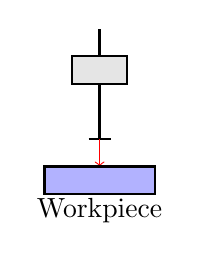
\begin{tikzpicture}[scale=0.7]
																																\draw[thick, fill=gray!20] (0,0) rectangle (1,0.5);
																																\draw[thick] (0.5,0.5) -- (0.5,1);
																																\draw[thick] (0.5,0) -- (0.5,-1);
																																\draw[thick] (0.3,-1) -- (0.7,-1);
																																\draw[->, red] (0.5,-1) -- (0.5,-1.5);
																																\node[red] at (0.5,-1.8) {Arc};
																																\draw[thick, fill=blue!30] (-0.5,-2) rectangle (1.5,-1.5);
																																\node at (0.5,-2.3) {Workpiece};
																															\end{tikzpicture}
																															\end{center>
																																\begin{itemize}
																																	\footnotesize
																																	\item MIG, TIG, Spot welding
																																	\item Wire feed, gas supply
																																	\item Water cooling sometimes
																																	\item Needs torch cleaning station
																																\end{itemize}
																																\end{block>
																																	
																																	\begin{block}{Dispensing Tools}
																																		\begin{center>
																																			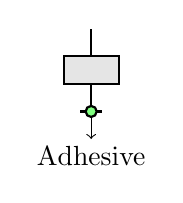
\begin{tikzpicture}[scale=0.7]
																																				\draw[thick, fill=gray!20] (0,0) rectangle (1,0.5);
																																				\draw[thick] (0.5,0.5) -- (0.5,1);
																																				\draw[thick] (0.5,0) -- (0.5,-0.5);
																																				\draw[thick] (0.3,-0.5) -- (0.7,-0.5);
																																				\draw[thick, fill=green!50] (0.5,-0.5) circle (0.1);
																																				\draw[->] (0.5,-0.6) -- (0.5,-1);
																																				\node at (0.5,-1.3) {Adhesive};
																																			\end{tikzpicture}
																																			\end{center>
																																				\begin{itemize}
																																					\footnotesize
																																					\item Glue, sealant, grease
																																					\item Metering pumps
																																					\item Need vision for path
																																					\item Cleanup important
																																				\end{itemize}
																																				\end{block>
																																					\end{column>
																																						
																																						\begin{column}{0.48\textwidth}
																																							\begin{block}{Spindle Tools}
																																								\begin{center>
																																									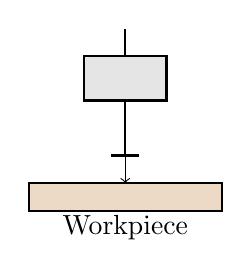
\begin{tikzpicture}[scale=0.7]
																																										\draw[thick, fill=gray!20] (0,0) rectangle (1.5,0.8);
																																										\draw[thick] (0.75,0.8) -- (0.75,1.3);
																																										\draw[thick] (0.75,0) -- (0.75,-1);
																																										\draw[thick] (0.5,-1) -- (1,-1);
																																										\draw[->] (0.75,-1) -- (0.75,-1.5);
																																										\node at (0.75,-1.8) {Tool rotation};
																																										\draw[thick, fill=brown!30] (-1,-2) rectangle (2.5,-1.5);
																																										\node at (0.75,-2.3) {Workpiece};
																																									\end{tikzpicture}
																																									\end{center>
																																										\begin{itemize}
																																											\footnotesize
																																											\item Drilling, milling, routing
																																											\item High-speed spindles
																																											\item Automatic tool changers
																																											\item Chip management
																																										\end{itemize}
																																										\end{block>
																																											
																																											\begin{block}{Other Common Tools}
																																												\begin{itemize}
																																													\footnotesize
																																													\item \textbf{Painting:} Spray guns, rotational atomizers
																																													\item \textbf{Deburring:} Rotary files, brushes
																																													\textbf{Measuring:} Probes, laser scanners
																																													\textbf{Material Handling:} Forks, magnets, hooks
																																													\textbf{Assembly:} Screwdrivers, nut runners
																																												\end{itemize}
																																												\end{block>
																																													\end{column>
																																														\end{columns>
																																														\end{frame}
																																														
																																														\begin{frame}{End Effector Selection Considerations}
																																															\begin{columns}
																																																\begin{column}{0.5\textwidth}
																																																	\begin{block}{Technical Factors}
																																																		\begin{itemize}
																																																			\item \textbf{Part geometry} and material
																																																			\item Required \textbf{gripping force}
																																																			\item \textbf{Cycle time} requirements
																																																			\item \textbf{Payload} capacity of robot
																																																			\item \textbf{Accuracy} and repeatability needs
																																																			\item \textbf{Environmental conditions}
																																																			\begin{itemize}
																																																				\footnotesize
																																																				\item Temperature
																																																				\item Cleanliness
																																																				\item Explosive atmosphere
																																																			\end{itemize}
																																																		\end{itemize}
																																																		\end{block>
																																																			\end{column>
																																																				
																																																				\begin{column}{0.5\textwidth}
																																																					\begin{block}{Economic \& Practical Factors}
																																																						\begin{itemize}
																																																							\item \textbf{Cost} of end effector
																																																							\item \textbf{Maintenance} requirements
																																																							\item \textbf{Changeover time} for different parts
																																																							\item \textbf{Reliability} and MTBF
																																																							\item \textbf{Vendor support}
																																																							\item \textbf{Integration complexity}
																																																						\end{itemize}
																																																						\end{block>
																																																							
																																																							\begin{alertblock}{Modern Trends}
																																																								\begin{itemize}
																																																									\footnotesize
																																																									\item \textbf{Adaptive grippers} (soft robotics)
																																																									\item \textbf{Force sensing} in fingers
																																																									\item \textbf{Vision-integrated} grippers
																																																									\item \textbf{Quick-change} systems
																																																									\item \textbf{Collaborative} (safe) grippers
																																																								\end{itemize}
																																																								\end{alertblock>
																																																									\end{column>
																																																										\end{columns>
																																																											
																																																											\vspace{5mm}
																																										

	\begin{exampleblock}{Rule of Thumb}
																																																														End effector weight should be \textbf{≤ 10\%} of robot's rated payload for optimal performance.
	\end{exampleblock}																																		
																																										\end{frame}
	\end{document}